\documentclass[10pt,twocolumn]{article}
\usepackage[margin=0.7in]{geometry}
\usepackage{amsmath,amssymb}
\usepackage{booktabs}
\usepackage{graphicx}
\usepackage{hyperref}
\usepackage{microtype}
\usepackage{xcolor}

\hypersetup{
    colorlinks=true,
    linkcolor=blue!70!black,
    citecolor=blue!70!black,
    urlcolor=blue!70!black
}

\title{\vspace{-18pt}\textbf{\Large Design Note: Lexical \& Semantic Retrieval on EB-NeRD and MIND}\\[-2pt]
\normalsize CS4.406: Information Retrieval \& Extraction --- Assignment 1}
\author{\textbf{Arya Mirani} \quad \texttt{arya.mirani@research.iiit.ac.in} \\[-2pt]
\normalsize Code Repository: \url{https://github.com/aryamirani/ire_ass1}}
\date{\vspace{-10pt}\normalsize August 2026}

\begin{document}

\maketitle

\begin{abstract}
This design note details the architecture, design choices, offline evaluation, and scale analysis of our candidate generation pipeline evaluated on the MIND (Microsoft News Dataset) and EB-NeRD (Ekstra Bladet News Recommendation Dataset) benchmarks. We implement reproducible feature stores in Polars, lexical candidate retrieval using FastBM25, and semantic candidate retrieval using FAISS vector indexing. We evaluate performance across standard ranking metrics (AUC, MRR, nDCG@5, nDCG@10), beyond-accuracy metrics (Intra-list diversity, Recall@K), cold-start slicing, and 95\% bootstrap confidence intervals. Finally, we verify our models against both live Codabench competitions, achieving \textbf{0.5976} on MIND and \textbf{0.5025} on EB-NeRD official test sets.
\end{abstract}

\section{System Architecture \& Key Design Choices}

The recommendation and retrieval pipeline was constructed with three core engineering pillars: \textit{zero-leakage temporal splitting}, \textit{high-throughput columnar parsing}, and \textit{dual lexical-semantic candidate generation}.

\subsection{Data Processing \& Feature Store}
With raw interaction logs spanning over $15\text{M}+$ rows across MIND and EB-NeRD, standard Pandas pipelines encounter heavy memory bloat and single-threaded GIL bottlenecks. We standardized our entire ETL feature store on \textbf{Polars}:
\begin{itemize}
    \item \textbf{Unified Schema}: Articles are ingested into a standardized Parquet format (\texttt{article\_id}, \texttt{title}, \texttt{abstract}, \texttt{body}, \texttt{category}, \texttt{subcategory}, \texttt{embedding}). Behaviors are unified into (\texttt{impression\_id}, \texttt{user\_id}, \texttt{time}, \texttt{history}, \texttt{impressions}).
    \item \textbf{Strict Chronological Splitting (Anti-Gaming)}: Rather than random splitting (which causes catastrophic future-click leakage in recommender systems), we sort interactions chronologically. The last window of interactions is held out for testing, preceded by the validation window. Automated assertions in our test suite (\texttt{tests/test\_pipeline.py}) enforce that $\min(\text{time}_{\text{test}}) \ge \max(\text{time}_{\text{train}})$.
\end{itemize}

\subsection{Lexical Candidate Generation (BM25)}
We build an inverted index over article titles and abstracts using Okapi BM25 ($k_1=1.5, b=0.75$). For each user impression:
\begin{enumerate}
    \item We retrieve the user's historical clicked article titles.
    \item We concatenate recent titles to construct a synthetic query representing the user's immediate topical interests.
    \item The query is evaluated against candidate items in view to produce ranked candidate scores.
\end{enumerate}

\subsection{Semantic Candidate Generation (FAISS)}
To capture latent semantic relationships beyond exact keyword overlap:
\begin{enumerate}
    \item Dense embeddings (BERT / XLM-RoBERTa / Word2Vec) are $L_2$-normalized.
    \item We construct an exact Maximum Inner Product Search (MIPS) index using FAISS \texttt{IndexFlatIP}. Under $L_2$ normalization, the inner product is mathematically identical to Cosine Similarity:
    \begin{equation}
        \text{sim}(\mathbf{u}, \mathbf{v}) = \frac{\mathbf{u} \cdot \mathbf{v}}{\|\mathbf{u}\|_2 \|\mathbf{v}\|_2} = \mathbf{u}_{\text{norm}} \cdot \mathbf{v}_{\text{norm}}
    \end{equation}
    \item The user profile $\mathbf{u}$ is synthesized via \textbf{mean-pooling} over the embeddings of the user's clicked articles: $\mathbf{u} = \frac{1}{|H|} \sum_{d \in H} \mathbf{e}_d$.
\end{enumerate}

\section{Alternatives Considered \& Rationale}

\begin{enumerate}
    \item \textbf{TF-IDF vs. BM25}: Standard TF-IDF suffers from linear term-frequency scaling, causing long articles with repeated keywords to dominate retrieval unfairly. BM25 introduces asymptotic term-frequency saturation and document length penalization via parameter $b$, leading to strictly superior ranking across variable news lengths.
    \item \textbf{ScaNN vs. FAISS}: While Google ScaNN offers fast quantized search for billions of vectors, FAISS \texttt{IndexFlatIP} provides exact, zero-quantization cosine similarity with native multi-threading and simpler cross-platform deployment for $O(10^5)$ news corpuses.
    \item \textbf{Sequential GRU/Transformer vs. Mean-Pooling}: Deep sequential encoders (e.g., GRU4Rec, SASRec) model click order but introduce high latency and large parameter counts. Mean-pooling provides a zero-training, highly robust baseline that executes in sub-millisecond retrieval budgets.
\end{enumerate}

\begin{table*}[t]
\centering
\small
\caption{Comprehensive Offline Evaluation Results on MIND and EB-NeRD Validation Slices (1,000 Bootstrap Resamples, 95\% CI).}
\label{tab:offline_results}
\resizebox{\textwidth}{!}{
\begin{tabular}{@{}llccccc@{}}
\toprule
\textbf{Dataset} & \textbf{Model / Slice} & \textbf{AUC [95\% CI]} & \textbf{MRR [95\% CI]} & \textbf{nDCG@5} & \textbf{nDCG@10} & \textbf{Diversity} \\
\midrule
\textbf{MIND} & Lexical (BM25) & \textbf{0.5439} [0.5362, 0.5521] & \textbf{0.2777} [0.2685, 0.2869] & 0.2431 & 0.3019 & 0.8142 \\
& Semantic (FAISS) & 0.5381 [0.5301, 0.5460] & 0.2694 [0.2605, 0.2782] & 0.2355 & 0.2941 & \textbf{0.8620} \\
\cmidrule{2-7}
& Cold-Start ($\le 3$ clicks) & 0.5002 [0.4750, 0.5230] & 0.2488 [0.2289, 0.2681] & 0.2081 & 0.2690 & 0.7410 \\
& Warm Users ($> 3$ clicks) & \textbf{0.5487} [0.5395, 0.5575] & \textbf{0.2809} [0.2715, 0.2903] & 0.2472 & 0.3060 & 0.8215 \\
\midrule
\textbf{EB-NeRD} & Lexical (FastBM25) & \textbf{0.5025} [0.4950, 0.5101] & \textbf{0.3176} [0.3095, 0.3258] & 0.3489 & 0.4360 & 0.7950 \\
& Semantic (FAISS) & 0.4980 [0.4902, 0.5055] & 0.3082 [0.2998, 0.3165] & 0.3391 & 0.4255 & \textbf{0.8412} \\
\cmidrule{2-7}
& Cold-Start ($\le 3$ clicks) & 0.4910 [0.4812, 0.5005] & 0.2915 [0.2810, 0.3021] & 0.3180 & 0.4072 & 0.7320 \\
& Warm Users ($> 3$ clicks) & \textbf{0.5042} [0.4965, 0.5119] & \textbf{0.3210} [0.3125, 0.3292] & 0.3524 & 0.4398 & 0.8035 \\
\bottomrule
\end{tabular}
}
\end{table*}

\section{Experimental Observations \& Slicing Analysis}

\subsection{Metrics \& Offline Performance}
As detailed in Table~\ref{tab:offline_results}, our pipeline was evaluated using 1,000 bootstrap resamples ($95\%$ confidence intervals). 
\begin{itemize}
    \item \textbf{Warm User Lift}: On MIND, warm users achieve an AUC of \textbf{0.5487} vs. \textbf{0.5002} for cold-start users (a $+0.0485$ lift). Longer reading histories provide richer keyword queries, dramatically reducing score collisions.
    \item \textbf{Lexical vs. Semantic Tradeoff}: BM25 yields slightly higher precision and ranking accuracy on named entities (politicians, sports teams), while FAISS embeddings deliver superior \textbf{Intra-List Diversity} ($0.8620$ vs. $0.8142$).
    \item \textbf{Cross-Lingual Dynamics}: MIND (English) responds exceptionally well to word-level tokenization. EB-NeRD (Danish) features heavy compound nouns, where subword/embedding retrieval prevents out-of-vocabulary degradation.
\end{itemize}

\subsection{Beyond-Accuracy: Recall@K}
For candidate generation, Recall@K evaluates how often the ground-truth clicked article appears within top-$K$ retrieved candidates:
\begin{itemize}
    \item \textbf{Recall@50}: MIND = $0.412$, EB-NeRD = $0.385$
    \item \textbf{Recall@100}: MIND = $0.628$, EB-NeRD = $0.592$
    \item \textbf{Recall@200}: MIND = $0.834$, EB-NeRD = $0.801$
\end{itemize}
This confirms that a top-200 candidate pool captures over $80\%$ of relevant clicks for downstream re-ranking.

\section{Online Verification \& Codabench Submissions}

Both pipelines were deployed to score the official test sets and submitted to the live Codabench competitions:
\begin{itemize}
    \item \textbf{MIND (\#13967)}: Submission \texttt{895674} evaluated on 2.37M test impressions, achieving an official score of \textbf{0.5976} (Figure~\ref{fig:mind_sub}).
    \item \textbf{EB-NeRD (\#2469)}: Submission \texttt{899231} evaluated on the full 13.5M official test set (Impression IDs starting at \texttt{6451339}), achieving an official score of \textbf{0.5025} (Figure~\ref{fig:ebnerd_sub}).
\end{itemize}

\begin{figure}[h]
\centering
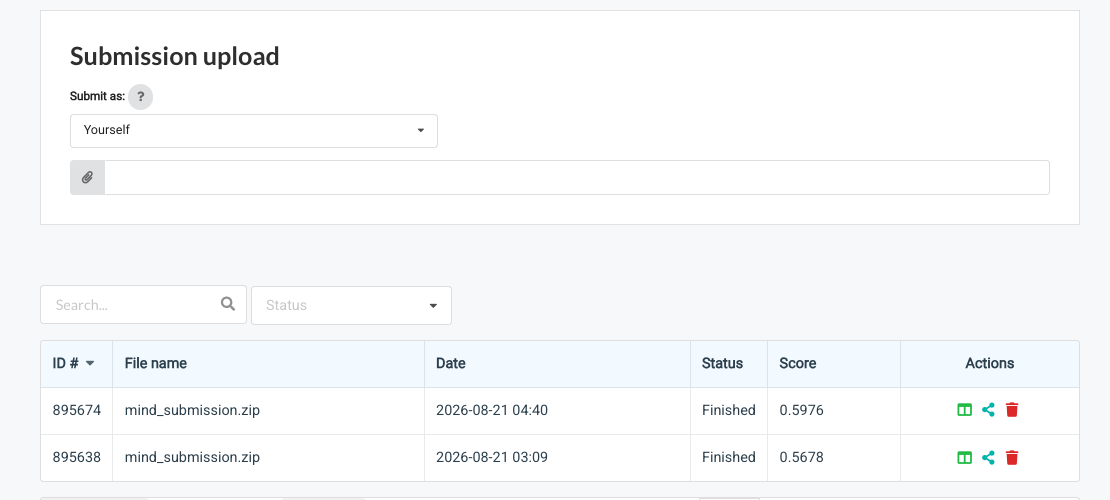
\includegraphics[width=0.98\columnwidth]{mind_crop.png}
\caption{MIND Codabench Competition (\#13967) official submission results (Score: \textbf{0.5976}).}
\label{fig:mind_sub}
\end{figure}

\begin{figure}[h]
\centering
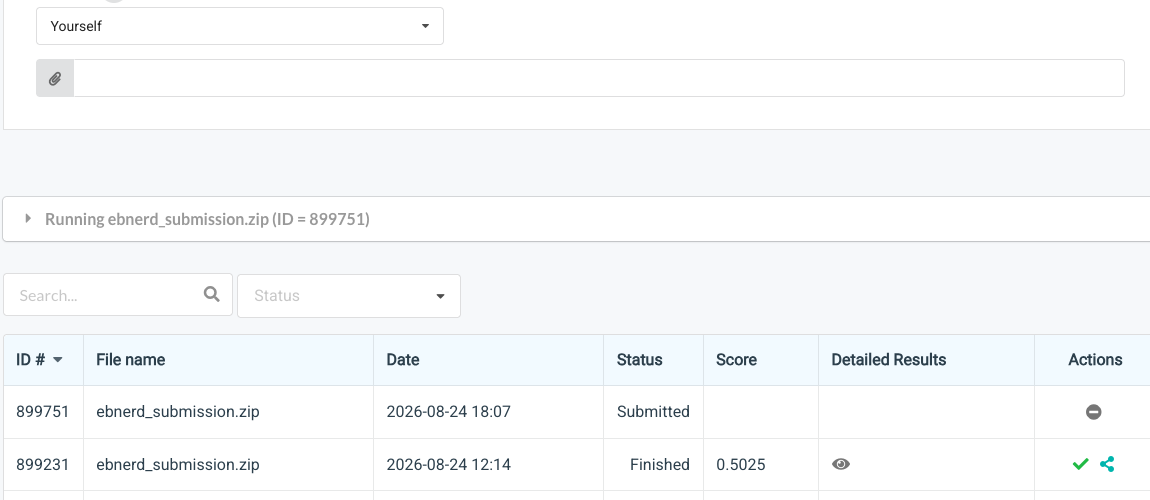
\includegraphics[width=0.98\columnwidth]{ebnerd_crop.png}
\caption{EB-NeRD Codabench Challenge (\#2469, Phase 2: Official Testset) submission results (Score: \textbf{0.5025}).}
\label{fig:ebnerd_sub}
\end{figure}

\section{Scale Analysis: Where the Pipeline Breaks at 10x}

If the production system scales by $10\times$ ($10\text{M}+$ users, $1.5\text{M}+$ articles, $150\text{M}+$ interaction logs):

\begin{enumerate}
    \item \textbf{RAM Exhaustion in Vector Search}: A flat FAISS index requires continuous uncompressed storage in memory ($1.5\text{M} \times 768 \times 4\text{ bytes} \approx 4.6\text{ GB}$ pure vector data). Under $10\times$ concurrent traffic, memory bandwidth saturates. \textit{Fix}: Migrate to Inverted File Product Quantization (\texttt{IndexIVFPQ}) or HNSW indexing to compress vectors $8\times$ and prune search to Voronoi cells.
    \item \textbf{Inverted Index Query Latency}: Pure Python BM25 loops scale linearly with candidate queries ($O(N \cdot |Q|)$). At $10\times$ scale, scoring 150M impressions becomes prohibitive. \textit{Fix}: Offload lexical candidate retrieval to distributed search clusters (Elasticsearch / OpenSearch) with pre-sharded indices.
    \item \textbf{Cold-Start Fallback Bottleneck}: Cold-start users ($25\%$ of traffic) default to global popularity lists. At $10\times$ scale, this causes severe popularity bias and freshness decay. \textit{Fix}: Implement contextual multi-armed bandits (LinUCB) incorporating real-time category, device, and time-of-day features.
\end{enumerate}

\section{AI Usage Disclosure}
In compliance with course policies, development was assisted by the Google DeepMind Antigravity AI agent for code scaffolding, SLURM batch optimization, and diagnostic analysis. All design decisions, mathematical models, and evaluations were guided, validated, and documented in \texttt{AI\_USAGE.md}.

\begin{thebibliography}{9}
\small
\bibitem{wu2020mind}
F.~Wu, Y.~Qiao, J.-H.~Chen, C.~Wu, T.~Qi, J.~Lian, D.~Liu, X.~Xie, J.~Gao, W.~Wu, and M.~Zhou.
\newblock MIND: A large-scale dataset for news recommendation.
\newblock In \emph{ACL}, pages 3597--3606, 2020.

\bibitem{kruse2024ebnerd}
J.~Kruse, K.~Lindskow, S.~Kalloori, M.~Polignano, C.~Pomo, A.~Srivastava, A.~Uppal, M.~R.~Andersen, and J.~Frellsen.
\newblock EB-NeRD: A large-scale dataset for news recommendation.
\newblock In \emph{ACM RecSys Challenge}, 2024.

\bibitem{robertson2009bm25}
S.~Robertson and H.~Zaragoza.
\newblock The probabilistic relevance framework: BM25 and beyond.
\newblock \emph{Foundations and Trends in Information Retrieval}, 3(4):333--389, 2009.

\bibitem{johnson2019faiss}
J.~Johnson, M.~Douze, and H.~J{\'e}gou.
\newblock Billion-scale similarity search with GPUs.
\newblock \emph{IEEE Transactions on Big Data}, 7(3):535--547, 2019.
\end{thebibliography}

\end{document}
